\documentclass{article}
%
%
%	brachistochrone.tex
%
%	David Meyer
%	dmm613@gmail.com
%	23 Sep 2022
%
%
%   get various packages
%
\usepackage[margin=1.0in]{geometry}                                     % adjust margins
\geometry{letterpaper}                                                  % or a4paper or a5paper or ... 
\usepackage{url}                                                        % need this to use URLs in bibtex
\usepackage{setspace}                                                   % need this for \setstrech{...}
\usepackage{scrextend}                                                  % need this for addmargin
\usepackage[export]{adjustbox}                                          % need this to get frame for includegraphics
%
%   tikz et al
%
\usepackage{tikz}
\usetikzlibrary{calc,patterns,angles,quotes,shapes,math,decorations,
                through,intersections,lindenmayersystems,backgrounds,
                hobby}
\tikzset{>=latex}                                                       % default to LaTeX arrow head
\usepackage{circuitikz}                                                 % draw circuits    
\usepackage{pgfplots}
%
%	more math stuff
%
\usepackage{amsmath,amsfonts,amssymb,amsthm}
\usepackage{mathtools}
\usepackage{commath}                                                    % get \norm{x}
\usepackage{fixmath}                                                    % get \mathbold
\usepackage{gensymb}                                                    % get \degree
\usepackage{mathrsfs}
\usepackage{hyperref}
\usepackage{subcaption}
\usepackage{authblk}
\usepackage{graphicx}
\usepackage{hyperref}
\usepackage{alltt}
\usepackage{color}
\usepackage{float}
\usepackage{braket}
\usepackage{siunitx}
\usepackage{relsize}
\usepackage{multirow}
\usepackage{esvect}
\usepackage{bigints}                                                    % bigger integral symbol
%
%	watermarks
%
% \usepackage{draftwatermark}
% \SetWatermarkText{Draft}
% \SetWatermarkScale{5}
% \SetWatermarkLightness {0.9} 
% \SetWatermarkColor[rgb]{0.7,0,0}
%
%
%	theorems, definitions, etc
%
\theoremstyle{definition}
\newtheorem{theorem}{Theorem}[section]
\newtheorem{definition}{Definition}[section]
\newtheorem{proposition}{Proposition}[section]
\newtheorem{lemma}{Lemma}[section]
\newtheorem{example}{Example}[section]
\newtheorem{remark}{Remark}[section]
%
%	The following code allows you to do
%
%	\begin{bmatrix}[r] (or [c] or [l])
%
\makeatletter
\renewcommand*\env@matrix[1][c]{\hskip -\arraycolsep
  \let\@ifnextchar\new@ifnextchar
  \array{*\c@MaxMatrixCols #1}}
\makeatother
%
%	make \arg{min,max}_{n \to \infty} work nicely
%
\newcommand{\argmax}{\operatornamewithlimits{argmax}}
\newcommand{\argmin}{\operatornamewithlimits{argmin}}
%
%	handy commands
%
\newcommand*{\Scale}[2][4]{\scalebox{#1}{$#2$}}
\DeclareMathOperator{\E}{\mathbb{E}}
\DeclareMathOperator{\bda}{\Big \downarrow}						% big down arrow
\newcommand{\veq}{\mathrel{\rotatebox{90}{$=$}}}
%
%	Title, author and date
%
\title{A Few Notes on the Brachistochrone Problem}
\author{David Meyer \\ \href{mailto:dmm613@gmail.com}
                            {dmm613@gmail.com}}
\date{Last Update: \today \\
	 {\vspace{1.00mm} \small Initial Version: January 8, 2022}}

%
%	be compatible
%
\pgfplotsset{compat=1.17} 
%
%
\begin{document}
\maketitle
%
%
%
\section{Introduction}
Johann Bernoulli posed the "problem of the brachistochrone" to the
readers of \emph{Acta Eruditorum} in June, 1696 \cite{1696acta}, 
which asks the following question:

\bigskip 
\begin{addmargin}[2em]{7em}                                                                             % 2em left, 7em right
Given two points $A$ and $B$ in a vertical plane, what is the
curve traced out by a point acted on only by gravity, which
starts at $A$ and reaches $B$ in the shortest time?  
\end{addmargin}


\bigskip
\noindent
The scenario Bernoulli envisioned is depicted in Figure
\ref{fig:brachistochrone}. 

\bigskip
\bigskip
%
%	brachistochrone problem setup
%
\begin{figure}[H]
  \centering
  \resizebox{0.80 \textwidth}{!} {                                                                      % resize the figure if you want
     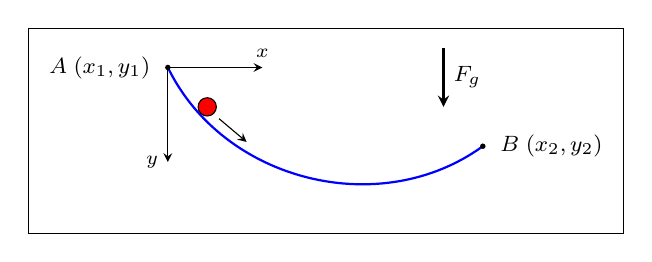
\begin{tikzpicture} [framed]                                                                       % draw the picture inside a black frame (requires \usetikzlibrary{backgrounds})
%
%	set up some coordinates
%
        \coordinate (A)		at (0.0,  0.0);								% put the origin at A
        \coordinate (Ax)	at (1.2,  0.0);								% x axis here
        \coordinate (Ay)	at (0.0, -1.2);								% y axis positive in the down direction
        \coordinate (Ball)	at (0.5, -0.5);								% draw the ball here
        \coordinate (B)		at (4.0, -1.0);								% other end of the curve
        \coordinate (Gy0)	at (3.5,  0.25);							% draw the gravity vector starting here
        \coordinate (Gy1)	at (3.5, -0.5);								% gravity vector ends here
        \coordinate (D0)	at (0.65,-0.65);							% draw motion arrow starting here
        \coordinate (D1)	at (1.0, -0.945);							% motion arrow ends here
%
%	draw the picture
%
        \draw[blue, thick] (A) to [bend right=50] (B);                 	% draw the curve in blue
        \node[circle, draw=black, fill=red, scale=0.70] at (Ball) {};	% draw a red ball with a black outline on the curve
        \draw[-stealth, thin] (D0) -- (D1);								% draw an arrow in the direction the ball is moving
        \fill (A) circle (0.035);										% put a dot on the curve at A
        \fill (B) circle (0.035);										% put a dot on the curve at B
        \draw[draw=none] (A) node[xshift=-0.10cm, font=\footnotesize, left] {$A \; (x_1,y_1)$};		% label A
        \draw[draw=none] (B) node[xshift=0.10cm, font=\footnotesize, right] {$B \; (x_2,y_2)$};		% label B
        \draw[-stealth, thin] (A) -- (Ax) coordinate [label={[font=\scriptsize, above] $x$}];		% draw x axis
        \draw[-stealth, thin] (A) -- (Ay) coordinate [label={[font=\scriptsize, left] $y$}];		% draw y axis
        \draw[-stealth, thick] (Gy0) -- (Gy1) coordinate [label={[font=\footnotesize, midway, right] $\vv{F_{g}}$}];	% draw the gravity vector (g)
      \end{tikzpicture}													% end \tikzipcture
    }                                                                                                   % end \resizebox
  \caption{The Brachistochrone Problem Setup}
  \label{fig:brachistochrone}
\end{figure}

\medskip
\section{A Bit of History}
\label{sec:history}
The problem posed by Johann Bernoulli was the called the
Brachistochrone\footnote{The word brachistochrone comes from the
Ancient Greek: \emph{brachis} (shortest) + \emph{chronos} (time)
\cite{enwikisource:6202943}.} problem, or the path of fastest
descent. Bernoulli issued his challenge in \emph{Acta Eruditorum}
\cite{1696acta}, writing

\bigskip
\begin{addmargin}[2em]{7em}
I, Johann Bernoulli, address the most brilliant mathematicians in
the world. Nothing is more attractive to intelligent people than
an honest, challenging problem, whose possible solution will
bestow fame and remain as a lasting monument. Following the
example set by Pascal, Fermat, etc., I hope to gain the gratitude
of the whole scientific community by placing before the finest
mathematicians of our time a problem which will test their
methods and the strength of their intellect. If someone
communicates to me the solution of the proposed problem, I shall
publicly declare him worthy of praise.
\end{addmargin}


\noindent
Bernoulli wrote the problem statement as:

\bigskip
\begin{addmargin}[2em]{7em}
Given two points A and B in a vertical plane, what is the curve
traced out by a point acted on only by gravity, which starts at A
and reaches B in the shortest time.
\end{addmargin}

\bigskip
\noindent
Figure \ref{fig:brachistochrone} attempts to capture Bernoulli's
problem statement.

\bigskip
\noindent
Galileo had attempted to solve this problem in his \emph{Two New
Sciences} \cite{wiki:two_new_sciences} and had concluded, based
on geometric arguments, that the solution was a circular
path. Galileo's approach is shown in Figure
\ref{fig:galileo}. Apparently Galileo hedged a bit on his
solution. In fact, it is said that he had reservations about his
conclusion and suggested that a “higher mathematics” would
possibly find a better solution \cite{brachistochrone_problem}.

\bigskip
\begin{figure}[H]
\center{\includegraphics[frame,scale=0.27] {images/galileo.png}}
\caption{Galileo considered a mass falling along different chords 
of a circle starting at A.  He proved that the path along ABG was
quicker than along AG, and ABCG was quicker than ABG, and ABCDG
was quicker than ABCG, etc.  In this way he showed that the path
along the circular arc was quicker than any set of chords. From
this he (incorrectly) inferred that the circle was the path of 
quickest descent. Galileo held out reservations about his
solution, and rightfully so.} 
\label{fig:galileo}
\end{figure}


\noindent
Then in 1659, while studying the physics of pendulums and time
keeping, Christiaan Huygens \cite{wiki:huygens} recognized that a
perfect harmonic oscillator, one whose restoring force was linear
in the displacement of the oscillator, would produce the perfect
time piece. Unfortunately, while the pendulum (as proposed by
Galileo) was the simplest oscillator to construct, Huygens knew
that it was not a perfect harmonic oscillator. In particular, he
knew that the period of oscillation became smaller when the
amplitude of the oscillation became larger. In order to “fix” the
pendulum, he searched for a curve of equal time, called the
\emph{tautochrone} \cite{wiki:tautochrone}, that would allow all
amplitudes of the pendulum to have the same period. He found the
solution and recognized it to be a cycloid \cite{wiki:cycloid}. 
The cycloid is shown in Figure \ref{fig:cycloid}.

\bigskip
\begin{figure}[H]
  \centering
  \resizebox{0.63 \textwidth}{!} {                                                                      % resize the figure if you want draw the picture
    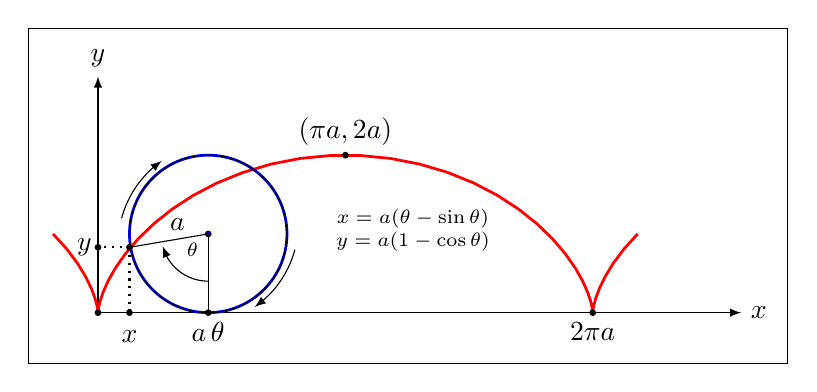
\begin{tikzpicture} [framed]                                                                        %  inside a black frame (requires
                                                                                                        %  \usetikzlibrary{backgrounds})
%
%       Define a few coordinates
%
     \coordinate (O) at (0,0);
     \coordinate (A) at (0,3);
     \def\r{1}  i                                                                                       % r is the radius
     \def\c{1.4}                                                                                        % c is the center
     \coordinate (C) at (\c, \r);

     \draw[-latex] (O) -- (A) node[anchor=south] {$y$};
     \draw[-latex] (O) -- (2.6*pi,0) node[anchor=west] {$x$};
     \draw[red, domain=-0.5*pi:2.5*pi, samples=50, line width=1] plot ({\x - sin(\x r)},{1 - cos(\x r)});
     \draw[blue, line width=1] (C) circle (\r);
     \draw[] (C) circle (\r);
%
%       set up some variables and coordinates
%
     \def\x{0.4}                                                                                        % x
     \def\y{0.83}                                                                                       % y
     \def\xa{0.3}                                                                                       % coordinate x for arc left
     \def\ya{1.2}                                                                                       % coordinate y for arc left
     \coordinate (X)     at (\x, 0 );
     \coordinate (Y)     at (0, \y );
     \coordinate (XY)    at (\x, \y );
     \node[anchor=north,yshift=-1.0mm] at (X) {$x$};
     \draw[fill=black] (O) circle (1pt);                                                                % draw a dot at the origin
     \draw[fill=blue]  (C) circle (1pt);                                                                % draw center of circle
     \draw[] (C) -- node[anchor=south] {\; $a$} (XY);                                                   % draw radius of the circle
     \coordinate (B) at (\c, 0);                                                                        % bottom of circle, radius to the bottom
     \draw[] (C) -- (B) node[anchor=north] {$a \, \theta$};
     \draw[fill=black] (B) circle (1pt);

%
%       projections of point XY
%
     \draw[thick, dotted] (XY) -- (X);
     \draw[fill=black] (X) circle (1pt);
     \draw[thick, dotted] (XY) -- (Y) node[anchor=east, xshift=0.5mm] {$\quad y$};
     \draw[fill=black] (Y) circle (1pt);

%
%       arc theta
%       start arc
%
     \coordinate (S) at (\c, 0.4);
     \draw[->] (S) arc (-90:-165:0.6);
     \node[xshift=-2mm, yshift=-2mm] at (C) {\scriptsize $\theta$};
%
%       arc above
%
     \coordinate (AA) at (\xa, \ya);
     \draw[-latex, rotate=25] (AA) arc (-220:-260:1.3);
%
%       arc below
%
     \def\xb{2.5}											% coordinate x for arc bottom
     \def\yb{0.8}											% coordinate y for arc bottom
     \coordinate (AB) at (\xb, \yb);
     \draw[-latex, rotate=-10] (AB) arc (-5:-45:1.3);   
     \draw[fill=black] (XY) circle (1pt);                                                               % draw XY dot
%
%       top label
%
     \coordinate (T) at (pi, 2);
     \node[anchor=south] at (T)  {$(\pi a, 2 a )$} ;
     \draw[fill=black] (T) circle (1pt);
%
%       equations
%
     \coordinate (E) at ( 4,1.2);
     \coordinate (F) at ( 4,0.9);
     \node[] at (E) {\scriptsize $x=a(\theta - \sin \theta)$};
     \node[] at (F) {\scriptsize $y=a(1 - \cos \theta)$};
%
%       label 2pi a
%
     \coordinate (TPA) at (2*pi, 0);
     \node[anchor=north] at (TPA) {$2 \pi a$};
     \draw[fill=black] (TPA) circle (1pt);								% draw a dot on the x axis at 2 \pi a

    \end{tikzpicture}
  }
 \caption{The Cycloid Curve}
 \label{fig:cycloid}
\end{figure}


\bigskip
\begin{figure}[H]
\center{\includegraphics[scale=0.60] {images/cycloid_coordinates.png}}
\caption{Finding the Coordinates of the Point D on a Cycloid}
\label{fig:cycloid_coordinates}
\end{figure}

\bigskip
\noindent
BTW, how are the cycloid's $(x,y)$ coordinates computed? Consider
the scenario depicted in Figure \ref{fig:cycloid_coordinates}
\cite{cycloid_coordinates}. To find the $(x,y)$ coordinates of
the point D we look at the distances involved. We can see from
the figure that  

\medskip
\begin{itemize}
 \item The x-coordinate is the length of OT minus the length of DB
 \item The y-coordinate is the length of CT minus the length of CB 
 (note that CT = $a$ is the radius of C)
 \item The length of an arc that is subtended by a central angle is 
       equal to the radius times the central angle
\end{itemize} 

\bigskip
\noindent
Now, since the distance that circle C has rolled must be equal to
the length of arc DT and the arc DT is equal to $a \theta$ we know
that $a\theta = \text{arc DT} = \text{OT}$. We also know from
trigonometry that $\text{DB} = a \sin \theta \text{ and } \text{CB}
= a \cos \theta$.  

\bigskip
\noindent
If we work out these lengths we see that

\begin{equation*}
\begin{array}{lllll}
x
&=& \text{OT - DB}   					&\qquad \qquad \qquad \mathrel{\#} \text{See Figure \ref{fig:cycloid_coordinates}} \\
[5pt]
&=& a\theta \; – \; a \sin \theta       &\qquad \qquad \qquad \mathrel{\#} \text{OT = radius times the central angle = $a \theta$ and DB $= a \sin \theta$} \\
[5pt]
&=& a (\theta \; – \; \sin \theta)      &\qquad \qquad \qquad \mathrel{\#} x = a (\theta – \sin \theta) \\
[10pt]
\hspace{-2em} \text{and} \\
[10pt]
y
&=& \text{CT - CB}                      &\qquad \qquad \qquad \mathrel{\#} \text{Figure \ref{fig:cycloid_coordinates}} \\
[5pt]
&=& a \; – \; a \cos \theta             &\qquad \qquad \qquad \mathrel{\#} \text{CT = $a$ and CB $= a \cos \theta$} \\
[5pt]
&=& a (1 \; – \; \cos \theta)           &\qquad \qquad \qquad \mathrel{\#} y = a (1 – \cos \theta) 
\end{array}
\end{equation*}

\bigskip
\noindent
So as we saw in Figure \ref{fig:cycloid}, $x = a (\theta – \sin
\theta)$ and $y = a (1 – \cos \theta)$. 


\bigskip
\noindent
Ok, back to the history. So almost thirty years later, during the
infancy of the infinitesimal calculus, the Tautochrone problem
was held up as a master example of an “optimal” solution whose
derivation should yield to the much more powerful and elegant
methods of the calculus. Jakob Bernoulli, Johann’s brother,
succeeded in deriving the Tautochrone problem in 1690 using the
calculus, using the term “integral” for the first time in print,
but it was not at first clear what other problems could yield in
a similar way. 

\bigskip
\noindent
Then, in 1696, Johann Bernoulli posed the Brachistrochrone
problem in the pages of \emph{Acta Eruditorum}.   

\subsection{A (Very) Brief Timeline of Brachistrochrone Related Events}

\bigskip

\begin{equation*}
\begin{array}{lll}
&\bullet \; 1638  & - \;\;\; \text{Galileo proposes arc of a circle as the least time solution (Figure \ref{fig:galileo})}             \\
&\bullet \; 1658  & - \;\;\; \text{Pascal puts forth a challenge involving finding the area under a segment of a cycloid}              \\
&\bullet \; 1659  & - \;\;\; \text{Huygens shows experimentally that the cycloid is the solution to the Tautochrone problem}           \\
&\bullet \; 1662  & - \;\;\; \text{Fermat's proposes the Principle of Least Time \cite{wiki:fermats_principle}}                        \\
&\bullet \; 1696  & - \;\;\; \text{Johann Bernoulli poses the Brachistrochrone problem in \emph{Acta Eruditorum} (edited by Leibniz)}  \\
&\bullet \; 1697  & - \;\;\; \text{Solutions provided by the Bernoulli brothers, L'H\^{o}pital, Leibniz, and Newton (anonymously)}     \\
&\bullet \; 1707  & - \;\;\; \text{Euler is born}                                                                                      \\
&\bullet \; 1726  & - \;\;\; \text{Euler completes his Ph.D under Johann Bernoulli}                                                    \\
&\bullet \; 1727  & - \;\;\; \text{Newton dies}                                                                                        \\
&\bullet \; 1755  & - \;\;\; \text{Lagrange, at age 19, finds an analytic solution to the Tautochrone problem}                         \\
&\bullet \; 1755  & - \;\;\; \text{Euler drops his own approach in favor of Lagrange's purely analytic approach}                       \\
&\bullet \; 1756  & - \;\;\; \text{Euler renames the subject the "Calculus of Variations" in \emph{Elementa Calculi Variationum} \cite{cov}}
\end{array}
\end{equation*}

\medskip
\section{The Calculus of Variations and the Brachistrochrone Problem}
\label{sec:cov}
Consider a definite integral that depends on an unknown function $y(x)$ and its derivative 
$y^{\prime}(x) = \frac{dy}{dx}$

\begin{equation}
I[y(x)] = \int_a^b F(y(x), y^{\prime}(x)) \; dx
\label{eqn:I[y]}
\end{equation}

\bigskip
\noindent
A typical problem in the Calculus of Variations involves finding
a particular function $y(x)$ that maximizes or minimizes the
integral $I[y(x)]$ (Equation \ref{eqn:I[y]}), subject to the
boundary conditions $y(a) = A$ and $y(b) = B$. The integral
$I[y(x)]$ is an example of a \emph{functional}, which (more
generally) is a mapping from a set of allowable functions to the
reals. We say that $I[y(x)]$ has an \emph{extremum} when
$I[y(x)]$ takes its maximum or minimum value. Note that we use
square brackets to indicate that $I$ is a functional (rather than
a function) and we frequently see $y(t)$ abbreviated as $y$ and
$I[y(x)]$ as $I[y]$ (or just $I$).

\subsection{The Euler-Lagrange Equation}
\label{subsec:euler-lagrange}
Let $C^k [a,b]$ denote the set of continuous functions defined on
the interval $a \leq x \leq b$ whose first $k$-derivatives are
also continuous on $a \leq x \leq b$. Now, suppose that $I[Y(x)]$
is an extremum of the functional

\medskip
\begin{equation*}
I[y(x)] = \int_a^b L(y(x), y^{\prime}(x)) \; dx
\end{equation*}

\bigskip
\noindent
that is defined defined on all functions $y(x) \in C^2 [a,b]$
such that $y(a) = A$ and $y(b) = B$.  Then its solution $Y(x)$
satisfies the second order ordinary differential equation


\bigskip
\begin{equation}
\dfrac{d}{dt} \left ( \dfrac{\partial L}{\partial y^{\prime}}
\right ) -  \dfrac{\partial L}{\partial y} = 0 
\label{eqn:euler-lagrange}
\end{equation}

\bigskip
\noindent
Equation \ref{eqn:euler-lagrange} is known as the Euler-Lagrange
equation (see \cite{notes:pola} for a proof of the Equation
\ref{eqn:euler-lagrange}). It is the constraint imposed by the
Euler-Lagrange equation that allows us to find the extremum of
the functional.



\bigskip
\noindent
Recall the Brachistochrone problem setup shown in Figure
\ref{fig:brachistochrone}.  Here we are trying to find the path
that takes the \emph{shortest time} from point $A$ to $B$. In the
language of the calculus of variations \cite{wiki:cov} the
Brachistochrone problem is to minimize the functional

\begin{equation*}
I[y] = \int_{0}^{t} dt
\end{equation*}

\bigskip
\noindent
Consider a curve over in which we call an differential segment of
the path $ds$. Then we know that the velocity of the ball (or
bead, in Bernoulli's original problem statement) is

\begin{equation}
V = \dfrac{ds}{dt}
\label{eqn:v}
\end{equation}

\bigskip
\noindent
Now, treating $\dfrac{ds}{dt}$ as a fraction\footnote{Care needs
to be taken when treating a derivative as a fraction.} we can see
from Equation \ref{eqn:v} that

\bigskip
\begin{equation*}
dt = \dfrac{ds}{V}
\end{equation*}

\bigskip
\noindent
and so 

\begin{equation}
I[y] = \int_{0}^{t} dt = \int_A^B \dfrac{ds}{V}
\label{eqn:I}
\end{equation}


\bigskip
{\setstretch{1.85} 
\noindent
Can we say more about $ds$? Well, if some function $f(x)$ is
differentiable in the neighborhood of $ds$ and if $ds$ is of
differential length ($ds \to 0$) then we can build a right
triangle on $f(x)$ with $ds$ as the hypotenuse. Then from
Pythagoras we know that $ds^2 = dx^2 + dy^2$ and so $ds =
\sqrt{dx^2 + dy^2} = \sqrt{1 + \left ( \dfrac{dy}{dx} \right )^2}
\; dx$.  This scenario is depicted in Figure
\ref{fig:pythagorean_theorem}.  \par}

\bigskip
%
%	draw Pythagorean theorem stuff
%
\begin{figure}[H]
\centering
  \resizebox{0.75 \textwidth}{!} {																							% resize figure if you want
  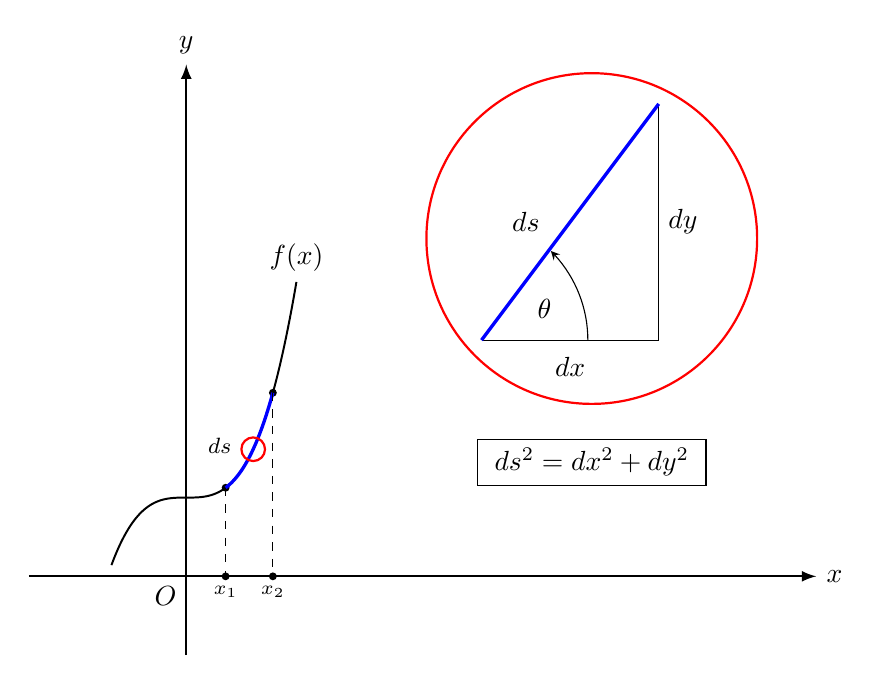
\begin{tikzpicture} [every edge quotes/.append style = {anchor=south, sloped},declare function={f(\x)=1 + \x*\x*\x;}]		% define f(x)
       \draw[thick, -latex] (-2,0) -- (8.0,0.0) coordinate [label={[right] $x$}];  											% x axis
       \draw[thick, -latex] (0,-1) -- (0,6.5) coordinate [label={[above] $y$}]; 											% y axis
       \draw [line width=0.25mm, smooth,samples=100,domain=-0.95:1.40] plot (\x,{f(\x)});									% draw f(x)
       \draw [draw=none] (1.40, {f(1.40)}) coordinate [label={[above] $f(x)$}];												% label f(x)
       \coordinate (O) at (0,0); 																							% origin
       \path (O) node[below left] {$O$};																					% draw origin
%
%	various coordinates
%     
       \coordinate (x1y1) at (0.5,{f(0.5)});
       \coordinate (x1y0) at (0.5,0.0);
       \coordinate (x2y2) at (1.1,{f(1.1});
       \coordinate (x2y0) at (1.1,0.0);
       \coordinate (cir)  at (0.85,{f(0.85)});
%
       \fill (x1y1) circle (0.05);																					% put a dot on the curve at x1y1
       \fill (x2y2) circle (0.05);																					% put a dot on the curve at x2y2
	   \draw [very thick,blue,smooth,samples=100,domain=0.5:1.1] plot (\x,{f(\x)});									% draw blue segment on f(x)
       \draw[draw=none] (x1y1) -- (x2y2) coordinate [label={[font=\footnotesize,yshift=-0.065cm,xshift=-0.105cm,midway,left] \color{black} $ds$}];
       \draw[dashed] (x1y1) -- (x1y0) coordinate [label={[font=\scriptsize,below] \color{black} $x_1$}];
       \draw[dashed] (x2y2) -- (x2y0) coordinate [label={[font=\scriptsize,below] \color{black} $x_2$}];
       \fill (x1y0) circle (0.05);																					% put a dot on the x axis at x1
       \fill (x2y0) circle (0.05);																					% put a dot on the x axis at x2
       \draw[red, thick] (cir) circle (0.150);																		% put a circle on f(x) where ds is
       

     
%
%	draw triangle and circle to show ds
%   
%
%
%	set up triangle coordinates
%
	   \coordinate (a) at (3.75,3.00);
	   \coordinate (c) at (6.00,3.00);
	   \coordinate (b) at (6.00,6.00);
%
%	draw the triangle
%	   
       \draw[] (a) -- (c) coordinate [label={[yshift=-0.1cm,midway,below] ${dx}$}];										% dx
       \draw[] (c) -- (b) coordinate [label={[midway,right] ${dy}$}];													% dy
       \draw[blue,very thick] (a) -- (b) coordinate [label={[xshift=-0.25cm,midway,left] \color{black} ${ds}$}];		% ds
       \draw[red,thick] (5.15,4.29) circle (2.10);																		% big circle
       \draw[draw=none] (0,0) -- (5.15,1.75)  node[draw,rectangle,below] {${\; ds^2 = dx^2 + dy^2 \;}$};				% draw the pythagorean theorem
%
%	draw the angle      
%       
       \node[xshift=-2mm, yshift=-2mm] at (4.75,3.60) {$\theta$};
       \draw[-stealth,thin] (5.10,3.00) arc (0:45:1.60cm);
%
%	done
%
     \end{tikzpicture}
    }																					 								% end resizebox                                                            
 \caption{$f(x)$, $ds$ and the Pythagorean Theorem}
 \label{fig:pythagorean_theorem}
\end{figure}


% \begin{figure}[H]
%  \centering
% \resizebox{0.30 \textwidth}{!} {																				% resize the figure if you want
%    \begin{tikzpicture}[framed]
%      \draw [red] (0,0) coordinate[] (a) --
%            	   (3,0) coordinate[] (c) --
%            	   (3,3) coordinate[] (b) -- cycle;
%       \draw[draw=none] (a) -- (c) coordinate [label={[yshift=-0.1cm,midway,below]					${dx}$}];    % dx
%       \draw[draw=none] (c) -- (b) coordinate [label={[xshift=0.025,midway,right]  				${dy}$}];    % dy
%       \draw[draw=none] (a) -- (b) coordinate [label={[xshift=-0.2cm,yshift=0.025cm,midway,left]	${ds}$}];    % ds
%    \end{tikzpicture}
%  }
% \caption{$ds^2 = dx^2 + dy^2$}
% \label{fig:pythagorean_theorem}
%\end{figure}

\bigskip
\noindent
Armed with this information we can solve for $ds$ in terms of $y^{\prime}$:

\begin{equation*}
\begin{array}{lllll}
ds^2
&=& dx^2 + dy^2   												&\qquad \qquad \qquad \mathrel{\#} \text{Pythagorean Theorem (Figure \ref{fig:pythagorean_theorem})} \\
[10pt]
&=& \left ( 1 + \dfrac{dy^2}{dx^2} \right ) dx^2				&\qquad \qquad \qquad \mathrel{\#} \text{factor out $dx^2$} \\
[12pt]
&=& \left ( 1 + \left (\dfrac{dy}{dx} \right )^2 \right ) dx^2	&\qquad \qquad \qquad \mathrel{\#} \text{group $\dfrac{dy}{dx}$} \\
[12pt]
&=& \left ( 1 + (y^{\prime})^2 \right ) dx^2					&\qquad \qquad \qquad \mathrel{\#} \text{$y^{\prime} = \dfrac{dy}{dx}$; note that here we're treating $\dfrac{dy}{dx}$ as a fraction}\\
[10pt]
&\Rightarrow& ds = \sqrt{1 + (y^{\prime})^2} \; dx				&\qquad \qquad \qquad \mathrel{\#} \text{take the square root of both sides}
\end{array}
\end{equation*}

\bigskip
\noindent
So now we know that 

\begin{equation}
ds = \sqrt{1 + (y^{\prime})^2} \; dx	
\label{eqn:ds}
\end{equation}

\bigskip
\noindent
Next, we know from the Law of Conservation of Energy \cite{conservation_of_energy}
that 

\medskip
\begin{equation*}
\begin{array}{lllll}
\dfrac{1}{2} mV^2 - mgy  
&=& 0										&\qquad \mathrel{\#} \text{$\dfrac{1}{2} mV^2$ is the kinetic energy and $mgy$ is the potential energy} \\
[10pt]
&\Rightarrow& \dfrac{1}{2} mV^2 = mgy		&\qquad \mathrel{\#} \text{add $mgy$ to both sides} \\
[10pt]
&\Rightarrow& \dfrac{1}{2} V^2 = gy			&\qquad \mathrel{\#} \text{cancel $m$} \\
[10pt]
&\Rightarrow& V^2 = 2gy						&\qquad \mathrel{\#} \text{multiply both sides by 2} \\
[10pt]
&\Rightarrow& V = \sqrt{2gy}				&\qquad \mathrel{\#} \text{take the square root of both sides}
\end{array}
\end{equation*}


\bigskip
\noindent
So now we know that

\begin{equation}
V = \sqrt{2gy}
\label{eqn:V}
\end{equation}


\bigskip
\noindent
and we can write $I[y]$ as follows

\begin{equation*}
\begin{array}{lllll}
I[y]
&=& {\displaystyle \mathlarger{\mathlarger{\int_A^B}} \dfrac{ds}{V}}
									&\qquad \qquad \mathrel{\#} \text{definition of $I[y]$ (Equation \ref{eqn:I})} \\
[15pt]
&=& {\displaystyle \mathlarger{\mathlarger{\int_A^B}} \dfrac{\sqrt{1 + (y^{\prime})^2}}{\sqrt{2gy}} dx}	
									&\qquad \qquad \mathrel{\#} \text{Equations \ref{eqn:ds} and \ref{eqn:V}} \\
[15pt]

&=& {\displaystyle \dfrac{1}{\sqrt{2g}} \mathlarger{\mathlarger{\int_A^B}} \sqrt{\dfrac{1 + (y^{\prime})^2}{y}} \; dx} 
									&\qquad \qquad \mathrel{\#} \text{pull $\dfrac{1}{\sqrt{2g}}$ out of integral, consolidate square root}
\end{array}
\end{equation*}

\medskip
\bigskip
\noindent
So now we have this expression for $I[y]$:

\medskip
\bigskip
\begin{equation*}
I[y] = \dfrac{1}{\sqrt{2g}} \mathlarger{\mathlarger{\int_A^B}}  \sqrt{\dfrac{1 + (y^{\prime})^2}{y}} \; dx
\end{equation*}

\medskip
\bigskip
\noindent
The Calculus of Variations is about finding a function (rather
than a point) that minimizes or maximizes some other
function. The other function, which takes a function as an
argument, is called a functional. Here $I[y]$ is the functional
and we want to find a function $L(y,y^{\prime})$ that minimizes
$I[y]$. $L(y,y^{\prime})$ looks like

\medskip
\begin{equation}
L(y,y^{\prime}) = \sqrt{\dfrac{1 + (y^{\prime})^2}{y}}
\label{eqn:L}
\end{equation}

\bigskip
\noindent
The last piece of machinery we need is the Beltrami Identity
\cite{wiki:beltrami_identity}, which is a special case of the
Euler–Lagrange equation where $\dfrac{\partial L}{\partial y} =
0$. In this case the Euler-Lagrange equation reduces to

\bigskip
\begin{equation}
L - y^{\prime} \dfrac{\partial L}{\partial y^{\prime}} = C
\label{eqn:beltrami}
\end{equation}

\bigskip
\noindent
where $C$ is some constant (see \cite{wiki:beltrami_identity} for
a derivation). Plugging Equation \ref{eqn:L} into Equation
\ref{eqn:beltrami} we get

\bigskip
\begin{equation}
\sqrt{\dfrac{1 + (y^{\prime})^2}{y}} - y^{\prime} 
\dfrac{\partial}{\partial y^{\prime}} 
\mathlarger{\mathlarger{\Bigg [}} \sqrt{\dfrac{1 + (y^{\prime})^2}{y}} \mathlarger{\mathlarger{\Bigg ]}} 
= C
\label{eqn:bel0}
\end{equation}


\bigskip
\noindent
Taking the partial derivative in Equation \ref{eqn:bel0} we get

\medskip
\begin{equation*}
\begin{array}{lllll}
\sqrt{\dfrac{1 + (y^{\prime})^2}{y}}  - y^{\prime} \cdot 
\Bigg [
  \dfrac{1}{\sqrt{y}} \cdot
  \bigg ( 
    \dfrac{1}{2} \Big (1 + (y^{\prime})^2 \Big )^{- \frac{1}{2}} 
    \cdot 2 y^{\prime} 
  \bigg )
\Bigg ]
= C							&\mathrel{\#} \text{power rule: $\dfrac{d}{dx} u^n = n u^{n-1} \dfrac{du}{dx}, \; u= 1 + (y^{\prime})^2, \; n = \dfrac{1}{2}$} \\
[15pt]
\Rightarrow \sqrt{1 + (y^{\prime})^2} - \dfrac{(y^{\prime})^2}{\sqrt{1 + (y^{\prime})^2}} = \sqrt{y} \cdot C
							&\mathrel{\#} \text{multiply both sides by $\sqrt{y}$, cancel 2 and $\dfrac{1}{2}$} \\
[15pt]
\Rightarrow 1 + (y^{\prime})^2 -(y^{\prime})^2 = \sqrt{y (1 + (y^{\prime})^2)} \cdot C
							&\mathrel{\#} \text{multiply both sides by $\sqrt{1 + (y^{\prime})^2}$} \\
[15pt]
\Rightarrow 1 = \sqrt{y (1 + (y^{\prime})^2)} \cdot C
							&\mathrel{\#} (y^{\prime})^2 - (y^{\prime})^2 = 0 \\
[15pt]
\Rightarrow 1 = y (1 + (y^{\prime})^2) \cdot C^2
							&\mathrel{\#} \text{square both sides} \\
[15pt]
\Rightarrow \dfrac{1}{C^2} = y + y (y^{\prime})^2
							&\mathrel{\#} \text{divide both sides by $C^2$, multiply though by $y$} \\
[15pt]
\text{Now, let } \dfrac{1}{C^2} = C_1 = y + y (y^{\prime})^2
							&\mathrel{\#} \text{define constant $C_1$} \\
[15pt]
\Rightarrow (y^{\prime})^2 = \dfrac{C_1 - y}{y}
							&\mathrel{\#} \text{solve for $(y^{\prime})^2$} \\
[15pt]
\Rightarrow y^{\prime} = \sqrt{\dfrac{C_1 - y}{y}}
							&\mathrel{\#} \text{take the square root of both sides} \\
[15pt]
\Rightarrow \dfrac{dy}{dx} = \sqrt{\dfrac{C_1 - y}{y}}
							&\mathrel{\#} y^{\prime} = \dfrac{dy}{dx} \\

\end{array}
\end{equation*}
						
\bigskip
\noindent
So know we know that 



\begin{equation*}
\begin{array}{lllll}
\dfrac{dy}{dx}
&=& \sqrt{\dfrac{C_1 - y}{y}}																		&\qquad \mathrel{\#} \text{previous derivation} \\
[15pt]
&\Rightarrow& dx = \sqrt{\dfrac{y}{C_1 -y}} \; dy													&\qquad \mathrel{\#} \text{solve for $dx$} \\
[15pt]
&\Rightarrow& x + C_2  = \mathlarger{\mathlarger{\mathlarger{\int}}} \sqrt{\dfrac{y}{C_1 -y}} \; dy	&\qquad \mathrel{\#} \text{integrate both sides}
\end{array}
\end{equation*}

\smallskip
\bigskip
\noindent
Now let $y = C_1 \sin^2 \theta$ so that
$dy = 2 \: C_1 \sin \theta \: \cos \theta \: d\theta$. 
Then

\medskip
\begin{equation*}
\begin{array}{lllll}
x + C_2
&=& \mathlarger{\mathlarger{\mathlarger{\int}}}	
\sqrt{\dfrac{C_1 \sin^2 \theta}{C_1 - C_1 \sin^2 \theta}} \cdot	2 \: C_1 \sin \theta \: \cos \theta \: d\theta
			&\qquad \mathrel{\#} \text{substitute for $y$ and $dy$} \\
[15pt]
&=& \mathlarger {\mathlarger{\mathlarger{\int}}}	
\sqrt{\dfrac{C_1 \sin^2 \theta}{C_1 (1 - \sin^2 \theta)}} \cdot	2 \: C_1 \sin \theta \: \cos \theta \: d\theta												
			&\qquad \mathrel{\#} \text{factor out $C_1$} \\
[15pt]
&=& \mathlarger{\mathlarger{\mathlarger{\int}}}	\sqrt{\dfrac{C_1 \sin^2 \theta}{C_1 \cos^2 \theta}}
\cdot 2 \: C_1 \sin \theta \: \cos \theta \: d\theta												
			&\qquad \mathrel{\#} \cos^2 \theta = 1 - \sin^2 \theta \\
[15pt]
&=& \mathlarger{\mathlarger{\mathlarger{\int}}}	\dfrac{\sin \theta}{\cos \theta}
\cdot 2 \: C_1 \sin \theta \: \cos \theta \: d\theta												
			&\qquad \mathrel{\#} \text{take square root, cancel $C_1$}\\
[15pt]
&=& 2 \; C_1 \mathlarger{\mathlarger{\mathlarger{\int}}} \sin^2 \theta \; d\theta												
			&\qquad \mathrel{\#} \text{cancel $\cos \theta$, factor out $2 \; C_1$}\\
[15pt]
&=& 2 \; C_1 \mathlarger{\mathlarger{\mathlarger{\int}}} \dfrac{1}{2} (1 - \cos 2\theta) \; d\theta												
			&\qquad \mathrel{\#} \text{$\cos 2 \theta = 1 - 2 \sin^2 \theta$ (double-angle trig identity)} \\
[15pt]
&=& C_1 \mathlarger{\mathlarger{\mathlarger{\int}}} (1 - \cos 2\theta) \; d\theta												
			&\qquad \mathrel{\#} \text{cancel $2$ and $\dfrac{1}{2}$} \\
[15pt]
&=& C_1 \mathlarger{\mathlarger{\mathlarger{\int}}} \; d\theta - 
C_1 \mathlarger{\mathlarger{\mathlarger{\int}}} \cos 2\theta \; d\theta									
			&\qquad \mathrel{\#} \text{integration is a linear operator} \\
[15pt]
&=& C_1 \theta - C_1 \left ( \dfrac{1}{2} \sin 2\theta \right )									
			&\qquad \mathrel{\#} \text{integrate} \\
[15pt]
&=& C_1 \theta - \dfrac{C_1}{2} \sin 2\theta									
			&\qquad \mathrel{\#} \text{simplify} \\
[15pt]
&\Rightarrow& 									
x + C_2  = C_1 \theta - \dfrac{C_1}{2} \sin 2\theta			
			&\qquad \mathrel{\#} x = C_1 \theta - \dfrac{C_1}{2} \sin 2\theta - C_2
\end{array}
\end{equation*}


\bigskip
\noindent
Given these results we can state the solution for the Brachistochrone 
problem:


\bigskip
\begin{equation}
x = C_1 \theta -  \dfrac{C_1}{2} \sin 2\theta - C_2
\label{eqn:cycloid_x}
\end{equation}

\bigskip
\noindent
and since $y = C_1 \sin^2 \theta$ (definition) and $\sin^2 \theta = \dfrac{1}{2} (1- \cos 2 \theta)$ 
(double-angle trig identity)


\bigskip
\begin{equation}
y = \dfrac{C_1}{2} \left ( 1 - \cos 2 \theta \right )
\label{eqn:cycloid_y}
\end{equation}

\smallskip
\bigskip
\noindent
Note that the constants $C_1$ and $C_2$ can be found from the 
boundary conditions.


\bigskip
\noindent
Finally, recall the cycloid shown in Figure \ref{fig:cycloid} (reproduced here):

\bigskip
\begin{figure}[H]
\center{\includegraphics[scale=0.40] {images/cycloid1.png}}
\caption{The Cycloid Curve}
\label{fig:cycloid1}
\end{figure}

\bigskip
\noindent
If we set $C_1 = 2 a$, $C_2 = 0$, and $\theta = \dfrac{\phi}{2}$
in Equations \ref{eqn:cycloid_x} and \ref{eqn:cycloid_y} we see
that 

\bigskip
\begin{equation*}
\begin{array}{lllll}
x 
&=& C_1 \theta -  \dfrac{C_1}{2} \sin 2\theta - C_2
			&\qquad \qquad \qquad \qquad \mathrel{\#} \text{Equation \ref{eqn:cycloid_x}} \\
[10pt]
&=& C_1 \theta -  \dfrac{C_1}{2} \sin 2\theta
			&\qquad \qquad \qquad \qquad \mathrel{\#} C_2 = 0 \\
[10pt]
&=& 2 a \theta -  \dfrac{2 a}{2} \sin 2\theta 									
			&\qquad \qquad \qquad \qquad \mathrel{\#} C_1 = 2a  \\
[10pt]
&=& 2 a \dfrac{\phi}{2} -  \dfrac{2 a}{2} \sin \Bigg [ 2 \left (\dfrac{\phi}{2} \right ) \Bigg ]
			&\qquad \qquad \qquad \qquad \mathrel{\#} \theta = \dfrac{\phi}{2} \\
[10pt]
&=& a \phi -  a \sin \phi 														
			&\qquad \qquad \qquad \qquad \mathrel{\#} \text{cancel $\dfrac{1}{2}$ and $2$} \\
[10pt]
&=& a (\phi -  \sin \phi) 														
			&\qquad \qquad \qquad \qquad \mathrel{\#} x = a (\phi -  \sin \phi) \\
\end{array}
\end{equation*}


\bigskip
\noindent
and

\bigskip
\begin{equation*}
\begin{array}{lllll}
y	
&=& \dfrac{C_1}{2} \left ( 1 - \cos 2 \theta \right )
			&\qquad \qquad \qquad \qquad \mathrel{\#} \text{Equation \ref{eqn:cycloid_y}} \\
[10pt]
&=& \dfrac{2a}{2} \left ( 1 - \cos 2 \theta \right )
			&\qquad \qquad \qquad \qquad \mathrel{\#} C_1 = 2 a \\
[10pt]
&=& \dfrac{2a}{2} \Bigg ( 1 - \cos \left [ 2 \left (\dfrac{\phi}{2} \right ) \right ] \Bigg )
			&\qquad \qquad \qquad \qquad \mathrel{\#} \theta = \dfrac{\phi}{2} \\
[10pt]
&=& a \left ( 1 - \cos \phi \right )
			&\qquad \qquad \qquad \qquad \mathrel{\#} y = a \left (1 - \cos \phi \right)
\end{array}
\end{equation*}


\bigskip
\noindent
So we see that Equations \ref{eqn:cycloid_x} and
\ref{eqn:cycloid_y} turn out to be the equations for a cycloid
(as we saw in Figures \ref{fig:cycloid} and \ref{fig:cycloid1})
and hence the "shortest time curve", that is, the solution to the
Brachistochrone problem, is a cycloid.

\section{Other Path Minimization Problems}
There are many path minimization problems we can solve with the
Calculus of Variations. Here are a few examples (WIP).

\subsection{Minimize the Distance (Pythagoras)}
{\setstretch{1.5} In Section \ref{subsec:euler-lagrange} we saw
that we can solve for a differential distance $ds$ on some curve
using the Pythagorean Theorem; this is shown in Figure
\ref{fig:pythagorean_theorem}. Note that this approach requires
that we treat $\dfrac{dy}{dx}$ as a fraction and as mentioned
above, care needs to be taken when doing this. That said, as we
saw above \par}



\begin{equation*}
\begin{array}{lllll}
ds^2
&=& dx^2 + dy^2   												&\qquad \qquad \qquad \mathrel{\#} \text{Pythagorean Theorem (Figure \ref{fig:pythagorean_theorem})} \\
[10pt]
&=& \left ( 1 + \dfrac{dy^2}{dx^2} \right ) dx^2				&\qquad \qquad \qquad \mathrel{\#} \text{factor out $dx^2$} \\
[12pt]
&=& \left ( 1 + \left (\dfrac{dy}{dx} \right )^2 \right ) dx^2	&\qquad \qquad \qquad \mathrel{\#} \text{group $\dfrac{dy}{dx}$} \\
[12pt]
&=& \left ( 1 + (y^{\prime})^2 \right ) dx^2					&\qquad \qquad \qquad \mathrel{\#} \text{$y^{\prime} = \dfrac{dy}{dx}$; here we're treating $\dfrac{dy}{dx}$ as a fraction}\\
[10pt]
&\Rightarrow& ds = \sqrt{1 + (y^{\prime})^2} \; dx				&\qquad \qquad \qquad \mathrel{\#} \text{take the square root of both sides}
\end{array}
\end{equation*}


\bigskip
\noindent
So to minimize the distance we want to solve the following integral: 

\bigskip
\begin{equation*}
I[y] = \int_{x_1}^{x_2} ds = \int_{x_1}^{x_2} \sqrt{1 + (y^{\prime})^2} \; dx
\end{equation*}	

\medskip
\subsection{Minimize the Time (Brachistochrone Problem)}
We saw above that $ds = \sqrt{1 + (y^{\prime})^2} \; dx$	
(Equation \ref{eqn:ds}) and $V = \sqrt{2gy}$ (Equation 
\ref{eqn:V}) so the integral we want to solve to find the 
curve that minimizes the time taken between two points $A$ 
and $B$ works out to be 

\bigskip
\begin{equation*}
I[y]
= \mathlarger{\mathlarger{\int_0^t}} dt = \mathlarger{\mathlarger{\int_A^B}} \dfrac{ds}{V} 
= \mathlarger{\mathlarger{\int_A^B}} \sqrt{\dfrac{1 + (y^{\prime})^2}{2gy}} \; dx
= \dfrac{1}{\sqrt{2g}} \mathlarger{\mathlarger{\int_A^B}} \sqrt{\dfrac{1 + (y^{\prime})^2}{y}} \; dx
\end{equation*}

\medskip
\subsection{Minimize the Energy (Catenary Problem)}
The Catenary Problem \cite{wiki:catenary} (also known as the
hanging chain problem) considers the shape of a chain hanging
from two stationary points where the only force acting on the
chain is gravity. In the problem setup $\rho$ is the density of
the chain, $g$ is the acceleration of gravity, and $A$ is the
constant cross sectional area of the chain.  Note that since the
units of $\rho$ are $\frac{\text{mass}}{\text{volume}}$ and
${\displaystyle \lim_{ds \to 0} \text{Volume} = \text{Area}}$,
$\rho A = m$ for a differential piece of the chain of length
$ds$.


\bigskip
\noindent
In the Catenary Problem the chain is assumed to be stationary so
the kinetic energy is zero. So the total energy is the just
potential energy $mgy$. So here $I[y]$ is


\bigskip
\begin{equation*}
I[y]
= \int_{x_1}^{x_2} mgy \; ds
= \int_{x_1}^{x_2} (\rho A) g y \: ds 
= \rho A g \int_{x_1}^{x_2} y \; ds 
= \rho A g\int_{x_1}^{x_2} y \; \sqrt{1 + (y^{\prime})^2} \; dx
\end{equation*}

\medskip
\subsection{Minimize the Lagrangian (Lagrange's Equations)}
This one is discussed in detail in \cite{notes:pola} but briefly
here $I[y]$ is the integral of the Lagrangian:


\bigskip
\begin{equation*}
I[y] = \int_{t_1}^{t_2} L(y(t),y(t)^{\prime}) \; dt
\end{equation*}


\bigskip
\noindent
\bigskip
Recall that for the case of Lagrangian mechanics 
the Lagrangian $L$ is defined to be

\begin{equation*}
L \equiv T - V
\end{equation*}

\bigskip
\noindent
where $T$ is an object's kinetic energy and $V$ 
is its potential energy. 
%
%
%
\section{Conclusions}
%
%
%
\section*{Acknowledgements}
%
%	LaTeX source on overleaf.com
%
\section*{\LaTeX Source}
\url{https://www.overleaf.com/read/vpwbqqpnjywj}
%
%	get a bibliography
%
%	Note:.bib files go in ~/Library/texmf/bibtex/bib with TeXShop (MacTeX).
%	You can also use an absolute path, e.g. \bibliography{/Users/dmm/papers/bib/qc}
%
\bibliographystyle{plain}
\bibliography{qc}
%
%	done
%
\end{document} 

